\chapter{МОДЕЛИ И АЛГОРИТМЫ}

\section{Основные понятия и определения}

Для исключения неоднозначного понимания основных терминов приведем основные определения, которые используются к работе в качестве основы.

\textit{Структурированный текст} --- текстовый файл, структурированный человеком или роботом по определенным правилам, утвержденным в международных стандартах. В сети к этой группе относятся $\approx 20\%$ файлов.

\textit{Неструктурированный текст} --- текстовый файл, не прошедший обработку с целью его структуризации. В сети к этой группе относятся $\approx 70\%$ файлов.

\textit{Полуструктурированный текст} --- текстовый файл, частично структурированный человеком или роботом. В сети к этой группе относятся $\approx 10\%$ файлов.

\textit{Интеллект} --- самообучаемая природная или искусственная система, решающая нестандартные задачи для адаптации к изменениям среды.

\textit{Универсальный искусственный интеллект} (ИИ) --- самообучаемый аппаратно-программный комплекс, решающий адаптивные и другие нестандартные задачи лучше, чем человек.

\textit{Специализированный искусственный интеллект} (СИИ) --- узко сфокусированный самообучаемый аппаратно-программный комплекс, решающий определенные нестандартные задачи лучше, чем человек.

\textit{Интеллектуальные лингвистические системы} --- программы, автоматизирующие процессы преобразования неструктурированного текста в структурированный и синтеза аннотации о полученном результате.

\textit{Онтология} --- кратное описание объекта или процесса, допускающее уточнение от концепции до программного кода.   

\textit{Ключевое слово} --- слово в тексте, способное в совокупности с другими ключевыми словами представлять текст

\section{Вспомогательные алгоритмы}

Для интеллектуальной обработки текста важным этапом является подготовка текста к его обработке. Например, если реализовывать алгоритмы основанные на подсчете количества слов, тогда важно отнести к одному слову все его формы (разные падежи, единственное и множественное число, разные времена, если это глагол и так далее). Эту задачу можно решить с помощью алгоритмов \textit{стемминга} и \textit{лемматизации}.

\textit{Стемминг} (Stemming) --- это процесс нахождения основы слова для заданного исходного слова (является частью процесса нормализации текста).
Основа слова необязательно совпадает с морфологическим корнем слова. \hyperref[itm:mathmodel]{[\ref{itm:mathmodel}]}. Такое нахождение основы слова происходит с помощью грубых отсечений словообразовательных морфем. Популярным алгоритмом стемминга (подходящим для английского, русского и других языков) является алгоритм Портера, основная идея которого заключается в том, что во всех языках содержится ограниченное количество словообразующих морфем и они используются согласно некоторым правилам, которые в этом алгоритме задаются вручную для каждого языка. Алгоритм Портера состоит из пяти шагов. На каждом из шагов рассматривается словообразующий суффикс и оставшаяся часть слова. Они проверяются на соответствие правилам, описанным для каждого шага, и отсекаются, если удовлетворяют этим правилам. Мартин Портер продолжил разрабатывать свой алгоритм и новую версию алгоритма называл \textit{Snowball} \hyperref[itm:snowball]{[\ref{itm:snowball}]}.


\textit{Лемматизация} (Lemmatization) --- это процесс преобразования слова в его базовую форму. Разница между стеммингом и лемматизацией заключается в том, что лемматизация учитывает контекст и преобразует слово в его значимую базовую форму, тогда как стемминг просто удаляет последние несколько символов, что часто приводит к неверному значению и орфографическим ошибкам. Лемматизация является более интеллектуальной обработкой и приводит слово с учетом его части речи. Например, рассмотрим слово \textbf{\textit{Caring}} (заботливый)
\begin{align*}
Caring &\xrightarrow{Lemmatization} Care \\
Caring &\xrightarrow{Stemming} Car
\end{align*} 
В случае лемматизации мы получим слово \textbf{\textit{Care}} (забота), а используя алгоритмы стемминга получим слово \textbf{\textit{Car}} (автомобиль).

Для того, чтобы проводить операции над словами требуется сначала выделить слова в тексте. Такой процесс называется \textit{токенизация} (tokenization). Разделение текста на слова это частный случай токенизации, когда в качестве токена (минимальной единицы) берется слово. В качестве токена можно взять предложение, абзац, слово, знак препинания и т.д. 

Удаление \quotes{стоп слов}. В естественных языках используются слова, которые не несут смысловой нагрузки и достаточно часто встречаются в тексте, что может повлиять на результаты алгоритмов, основывающихся на расчете частоты появления слов в тексте. Примеры таких слов в английском языке: \textit{a}, \textit{the}, \textit{is}, \textit{are}. Также если рассматривать научные статьи, то ссылки на источники могут являться \quotes{стоп словами}.

\section{Модели}

Для формирования общей картины анализа текстов с прагматической точки зрения построим концептуальные модели сцены и ее участников, допускающие уточнение до уровня программного кода.

Модель сцены представим онтологией:
\begin{equation}
\label{eq:scene}
scene = (source, textIn, sys, textOut, Database, user)
\end{equation}
где: $source$ --- источник входных документов (файлов); $textIn$ --- входной файл; $sys$ система обработки; $textOut$ --- выходной файл; $Database$ --- база данных для хранения данных; $user$ --- пользователь базы.

Модель искомой системы представим онтологией:
\begin{equation}
\label{eq:system}
sys = (mControl, mIn, mProc, mDao, mVis)
\end{equation}
где: $mControl$ --- управляющая программа; $mIn$ --- модуль чтения входного текстового файла; $mProc$ --- модуль обработки; $mWrite$ --- модуль для работы с базой данных; $mVis$ --- модуль графического интерфейса.


Модель структурированного документа:
\begin{equation}
mStruct = (keywords, summary, document)
\end{equation}
где: $keywords$ --- ключевые слова этого документа; $summary$ --- реферат документа; $document$ --- исходный текст документа.

\section{Алгоритмы}

\subsection{Макро алгоритм}

Прежде всего разработаем общую схему обработки текста. Предлагается следующий вариант:

\begin{enumerate}
    \item на вход поступает текстовый документ $textIn$;
    \item сохраняем текстовый документ на диск;
    \item проверяем, существует ли запись об этом документе в базе данных;
    \item если записи не существует, переходим к следующему шагу, иначе --- сохраняем документ в базу;
    \item строим аннотацию и прибавляем ее к тексту;
    \item запись исходного и обработанного текста в $Database$.
\end{enumerate}

Рассмотрим подробнее алгоритмы построения аннотации для входного текста $textIn$. 

\subsection{Алгоритм составления реферата текста на основе алгоритма TextRank}\label{sec:textrank}

Для нахождения важности страниц в интернете используется алгоритм $PageRank$, суть которого заключается в следующем: на страницы, которые являются самыми важными ссылаются другие страницы. И если мы представим эту сеть как направленный взвешенный граф, вершины которого --- веб страницы, а ребра между вершинами $i$ и $j$ имеют вес равный количеству ссылок со страницы $i$ на страницу $j$. Тогда вычисляя сумму весов всех ребер, входящих в вершину, мы сможем найти вес вершины. Исходя из предположения, что на самые важные страницы ссылаются больше всего, можно сделать вывод, что страницы, представленные вершинами графа с самым большим весом являются самыми важными.

Алгоритм $TextRank$ является алгоритмом экстрактивной суммаризации (алгоритмом, который выделяет самые важные предложения из текста) основан на описанном выше алгоритме $PageRank$ \hyperref[itm:textrank]{[\ref{itm:textrank}]}. Вершинами графа в такой модели будут предложения и, в отличие от оригинального алгоритма, для определения веса используется модель неориентированного графа, а веса ребер отражают похожесть предложений в каком-то смысле.

Мной был предложен следующий алгоритм нахождения расстояния между предложениями:
\begin{enumerate}
    \item разбить предложение на слова;
    \item привести слова к нормальной форме (произвести лемматизацию);
    \item составить словарь $D$ содержащий слова из двух предложений без повторений;
    \item представить каждое предложение как $n$-мерный вектор, где $n$ --- размер словаря, $i$-ая компонента которого --- количество вхождений $i$-ого слова из словаря $D$;
    \item найти косинусное расстояние между этими векторами.
\end{enumerate} 

Вычислить косинусное расстояние между двумя векторами в $n$-мерном пространстве можно как косинус угла $\theta$ (рисунок \hyperref[fig:cosine]{\ref{fig:cosine}}) после представления этих векторов в полярных координатах.

\begin{figure}[H]
\centering
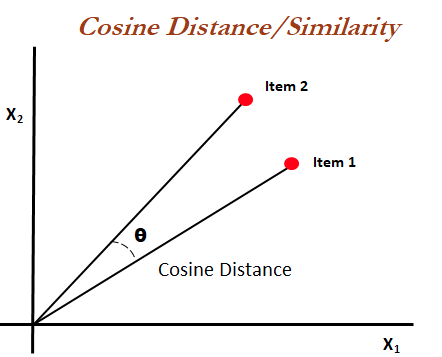
\includegraphics[width=0.6\textwidth]{cosine_distance.png}
\caption{Косинусное расстояние в двумерном пространстве}
\label{fig:cosine}
\end{figure}

Для нахождения косинусного расстояния в декартовых координатах можно воспользоваться следующей формулой:
\begin{equation}
distance(\vec{a}, \vec{b}) = \dfrac{(\vec{a}, \vec{b})}{||\vec{a}|| \cdot ||\vec{b}||} = \dfrac{\sum\limits_{i=1}^{n}a_i b_i}{\sqrt{\sum\limits_{i=1}^{n} a_i^2}\sqrt{\sum\limits_{i=1}^{n} a_i^2}}
\end{equation}

Следующим шагом является нахождение матрицы расстояний между всеми предложениями и составление графа текста. После составления графа можно посчитать вес каждого предложения и выбрать несколько предложений с наибольшим весом (экспериментально было выяснено, что это количество приблизительно равно $20\%$ от количества предложений в исходном тексте). Эти предложения можно считать рефератом текста.

\subsection{Эвристический алгоритм выделения ключевых слов}

\subsubsection{Закон Ципфа}

В 1949 году Джордж Ципф сформулировал несколько закономерностей \hyperref[itm:zipf]{[\ref{itm:zipf}]}. Данные законы получены не на основе математических выводов, а на
основе анализа статистики частоты слов текстах на многих языках, то есть эмпирически.
Если все слова достаточно длинного текста упорядочить по убыванию
частоты их использования, то частота $n$-го слова в таком списке окажется
приблизительно обратно пропорциональна его порядковому номеру $n$ (так
называемому рангу этого слова). Например, второе по используемости
слово встречается примерно в два раза реже, чем первое, третье — в три
раза реже, чем первое, и т. д. (рисунок \hyperref[fig:hips_rus]{\ref{fig:hips_rus}}).
\begin{figure}[H]
\centering
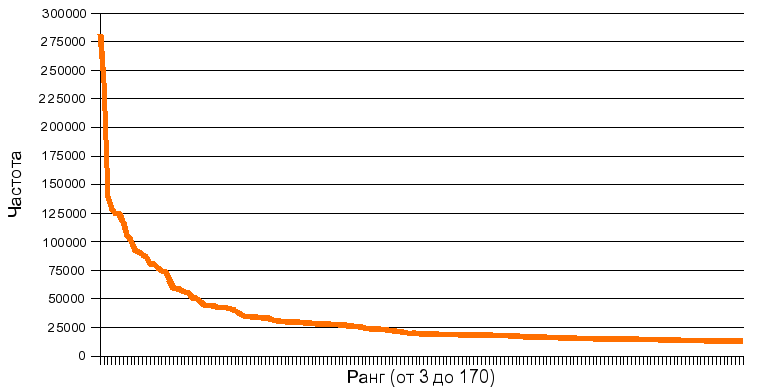
\includegraphics[width=0.6\textwidth]{hips_russian.png}
\caption{Закон Ципфа для русской Википедии}
\label{fig:hips_rus}
\end{figure}
Это утверждение верно в пределах одного языка. Однако и межъязыковые различия невелики. На каком бы языке текст ни был написан, вид
кривой Ципфа останется неизменной. Может немного отличаться лишь коэффициент гиперболы (рисунок \hyperref[fig:hips_diff]{\ref{fig:hips_diff}})
\begin{figure}[H]
\centering
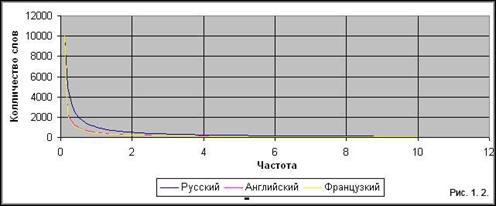
\includegraphics[width=0.6\textwidth]{hips_diff.png}
\caption{Закон Ципфа для разных языков}
\label{fig:hips_diff}
\end{figure}
Законы Ципфа позволяют находить ключевые слова.
Исследования показывают, что наиболее значимые для текста слова
лежат в средней части графика. Этот факт имеет простое обоснование. Слова, которые попадаются слишком часто, в основном оказываются предлогами, местоимениями. Редко встречающиеся слова тоже, в большинстве случаев, не имеют решающего смыслового значения \hyperref[itm:boyarsky]{[\ref{itm:boyarsky}]}.

\subsubsection{Идея алгоритма}

Следующий алгоритм содержит в себе идею, что слова, которые являются ключевые для какого-то текста используются чаще всего. Однако, если не применять эвристики и просто считать количество вхождений слова в предложении, то можно ошибочно посчитать предлоги, артикли и другие слова, не несущие смысловой нагрузки ключевыми словами. Поэтому перед выделением ключевых слов с помощью вычисления частоты появления слова в тексте необходимо сначала отфильтровать \quotes{стоп слова}. Для того, чтобы не рассматривать разные формы одного слова как разные слова, необходимо привести все слова в предложении к нормальной форме.

Далее на основании полученных частот слов и закона Ципфа, сортируем ключевые слова по убыванию частоты их использования и берем часть диапазона, ближайшую к началу (так как мы удалили большинство \quotes{стоп слов}). Для текстов малого объема при удалении стоп слов смещение диапазона для выбора ключевых слов не требуется, так как этот текст содержит небольшое количество связующих слов и вероятность того, что эти связующие слова не будут в списке известных стоп слов достаточно мала.

Итак, получим следующий алгоритм:
\begin{enumerate}
\item выделить в тексте слова;
\item удалить \quotes{стоп слова};
\item привести слова к нормальной форме с помощью лемматизации;
\item найти количество появлений каждого слова в тексте;
\item выбрать ключевые слова пропустив некоторое количество самых популярных слов в тексте, если текст достаточного объема.
\end{enumerate}

\subsection{Алгоритм выделения ключевых слов на основе алгоритмов машинного обучения}

Этот алгоритм также строится на предположении, что ключевые слова встречаются в тексте чаще всего. Однако, слова, которые встречаются во всех документах вряд ли могут быть ключевыми, так как не относятся к одной конкретной теме. Поэтому для выделения ключевых слов мной была использована модель $TF*IDF$.

\subsubsection{Модель TF*IDF}

Для понижения значимости слов, которые встречаются почти во всех документах, вводят инверсную частоту термина $IDF$
(inverse document frequency) — это логарифм отношения числа всех документов $D$ к числу документов $d$, содержащих некоторое слово.
\begin{equation}
\label{eq:idf}
IDF = \lg \dfrac{D}{d}
\end{equation}
Значение этого параметра тем меньше, чем чаще слово
встречается в документах коллекции. Таким образом, для слов, которые
встречаются в большом числе документов, $IDF$ будет близок к нулю (если
слово встречается во всех документах $IDF$ равен нулю), что помогает выделить важные слова.
Параметр $TF$ (term frequency) — это отношение числа раз $k_i$, которое
некоторое слово встретилось в документе, к общему числу слов в документе $n$. Нормализация длиной документа нужна для того, чтобы уравнять в правах короткие и длинные документы.
\begin{equation}
\label{eq:tf}
TF = \dfrac{k_i}{n}
\end{equation}
Коэффициент $TF*IDF$ равен произведению $TF$ и $IDF$, при этом $TF$ играет роль повышающего множителя, $IDF$ --- понижающего \hyperref[itm:datamining]{[\ref{itm:datamining}]}.

\subsubsection{Алгоритм выделения ключевых слов}

Алгоритм заключается в том, что при нахождении ключевых слов для каждого документа, документ добавляется в базу данных и в последующем используется для вычисления понижающего коэффициента $IDF$. Формально алгоритм можно записать следующим образом:
\begin{enumerate}
\item на вход поступает документ $textIn$ и искомое количество ключевых слов $k$;
\item в модель загружаются все документы из базы данных;
\item для каждого слова вычисляются коэффициенты $TF$ и $IDF$ по формулам \hyperref[eq:tf]{(\ref{eq:tf})} и \hyperref[eq:idf]{(\ref{eq:idf})};
\item вычисляется вес каждого слова по формуле $weight = TF*IDF$;
\item слова сортируются по убыванию веса;
\item выбираются первые $k$ слов;
\item документ сохраняется в базе данных.
\end{enumerate}

\subsection{Сравнительный анализ алгоритмов выделения ключевых слов}

Рассмотрим результаты работы алгоритмов, описанных выше на тексте, представленном в приложении \hyperref[app:capitalism]{\ref{app:capitalism}}. Были получены следующие результаты. Ключевые слова, полученные эвристическим алгоритмом: market, capitalism, capitalist, free. Эти слова являются чаще всего употребляемыми, но не дают полного представления о тексте. Рассмотрим результат работы алгоритма $TF*IDF$, обученного на книгах из открытого источника: capitalism, capitalist, economic, ownership. Такие ключевые слова являются более подходящими для этой статьи. Эти результаты обоснованы тем, что в качестве обучающей выборки была выбрана художественная литература, и слова, относящиеся к теме капитализма, являются незнакомыми для алгоритма, использующего машинное обучение.

Заметим, что оба эти алгоритма не подходят для анализа художественных текстов, в которых описываются действия, так как порядок слов в тексте не учитывается, результат работы алгоритмов будет неудовлетворительный. Рассмотрим это утверждение на примере приложения \hyperref[app:harry]{\ref{app:harry}}. В качестве ключевых слов алгоритмами были выбраны имена собственные, которые упоминаются чаще всего.

\section{Выводы}

Во второй главе были получены следующие результаты:
\begin{itemize}
\item разработана унифицированная модель сцены анализа текстов, основанная на анализе и обобщении сцен решения прикладных задач;
\item разработан алгоритм суммаризации на основе алгоритма TextRank;
\item разработан эвристический алгоритм выделения ключевых слов;
\item разработан алгоритм выделения ключевых слов на основе модели $TF*IDF$.
\end{itemize}
\newpage
